\section{Инструкция по работе с сайтом ОФД} \label{5500}
\begin{itemize}	
	\item В адресной строке браузера набрать адрес офд . Позиция 1 на (Рис.~\ref{ris:13.jpg})
	
	
	\begin{figure}[H]
		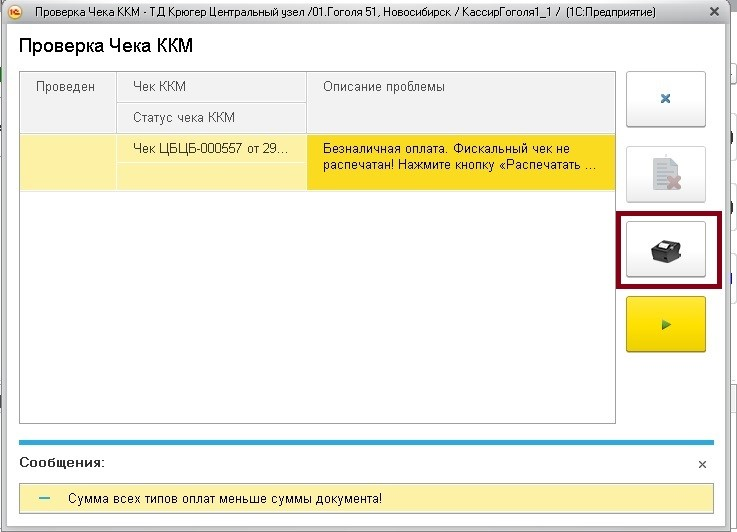
\includegraphics[width=1.0\textwidth]{13.jpg}
		\caption{<<Сайт ОФД>>.}
		\label{ris:13.jpg}
	\end{figure}

	\item Нажать «Войти в личный кабинет». Позиция 2 на на (Рис.~\ref{ris:13.jpg})

%{
%  \centering
%  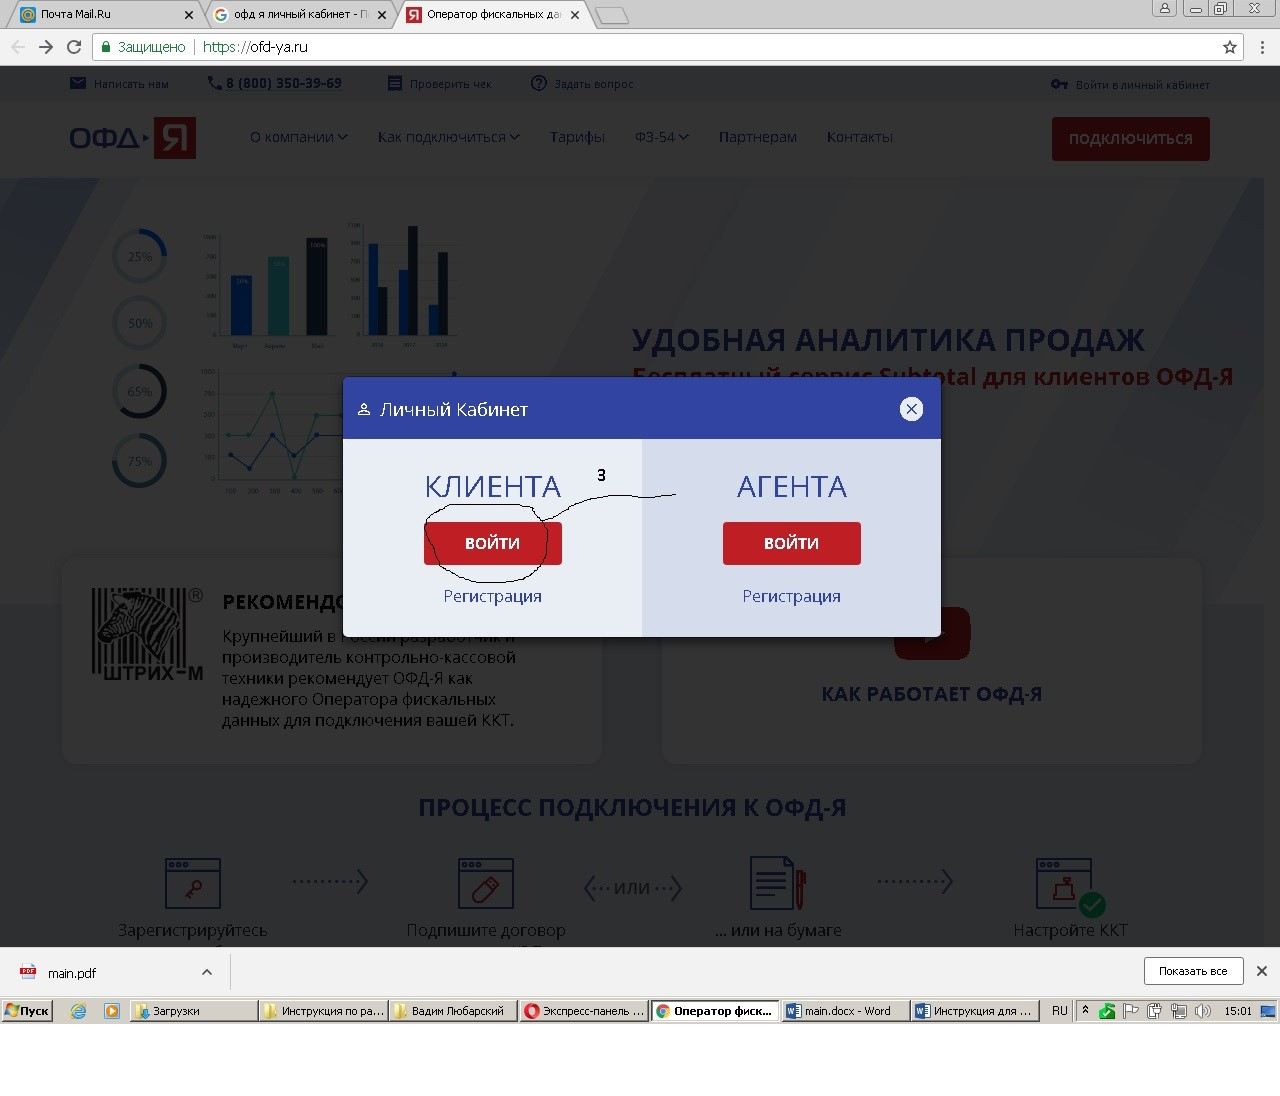
\includegraphics[width=1.0\textwidth]{14.jpg}
%  \captionof{figure}{<<Личный кабинет>>.}\label{ris:14.jpg}
%  }

	\begin{figure}[H]
		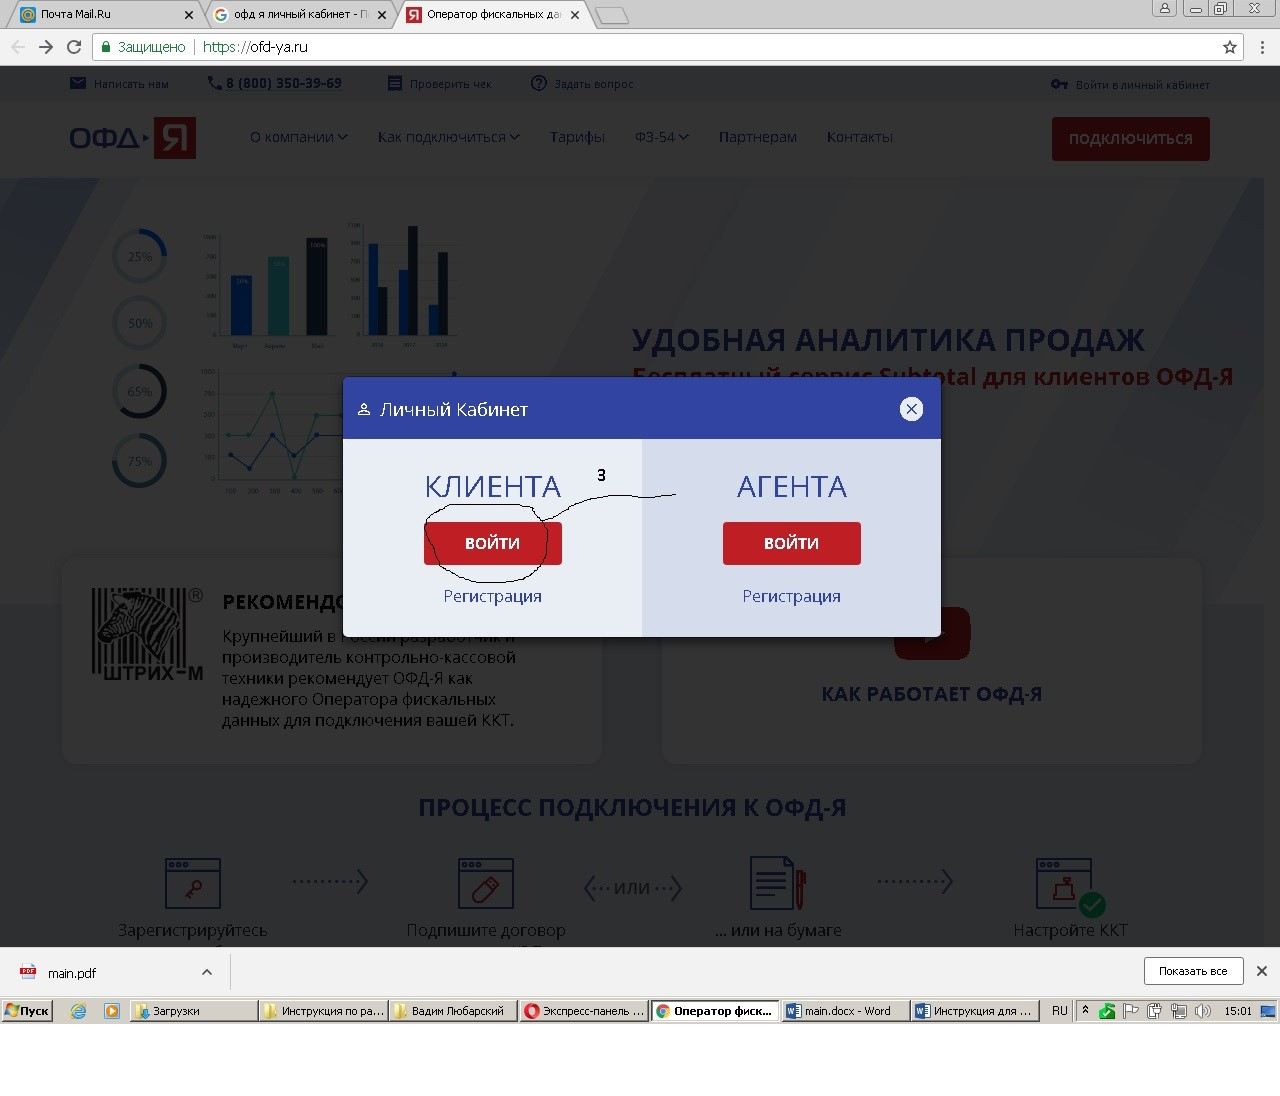
\includegraphics[width=1.0\textwidth]{14.jpg}
		\caption{<<Личный кабинет>>.}
		\label{ris:14.jpg}
	\end{figure}
	
	
	\item Нажать кнопку «войти». Позиция 3 на (Рис.~\ref{ris:14.jpg})
	
	\item Набрать логин и пароль. (Рис.~\ref{ris:15.jpg})
	
	\begin{figure}[H]
		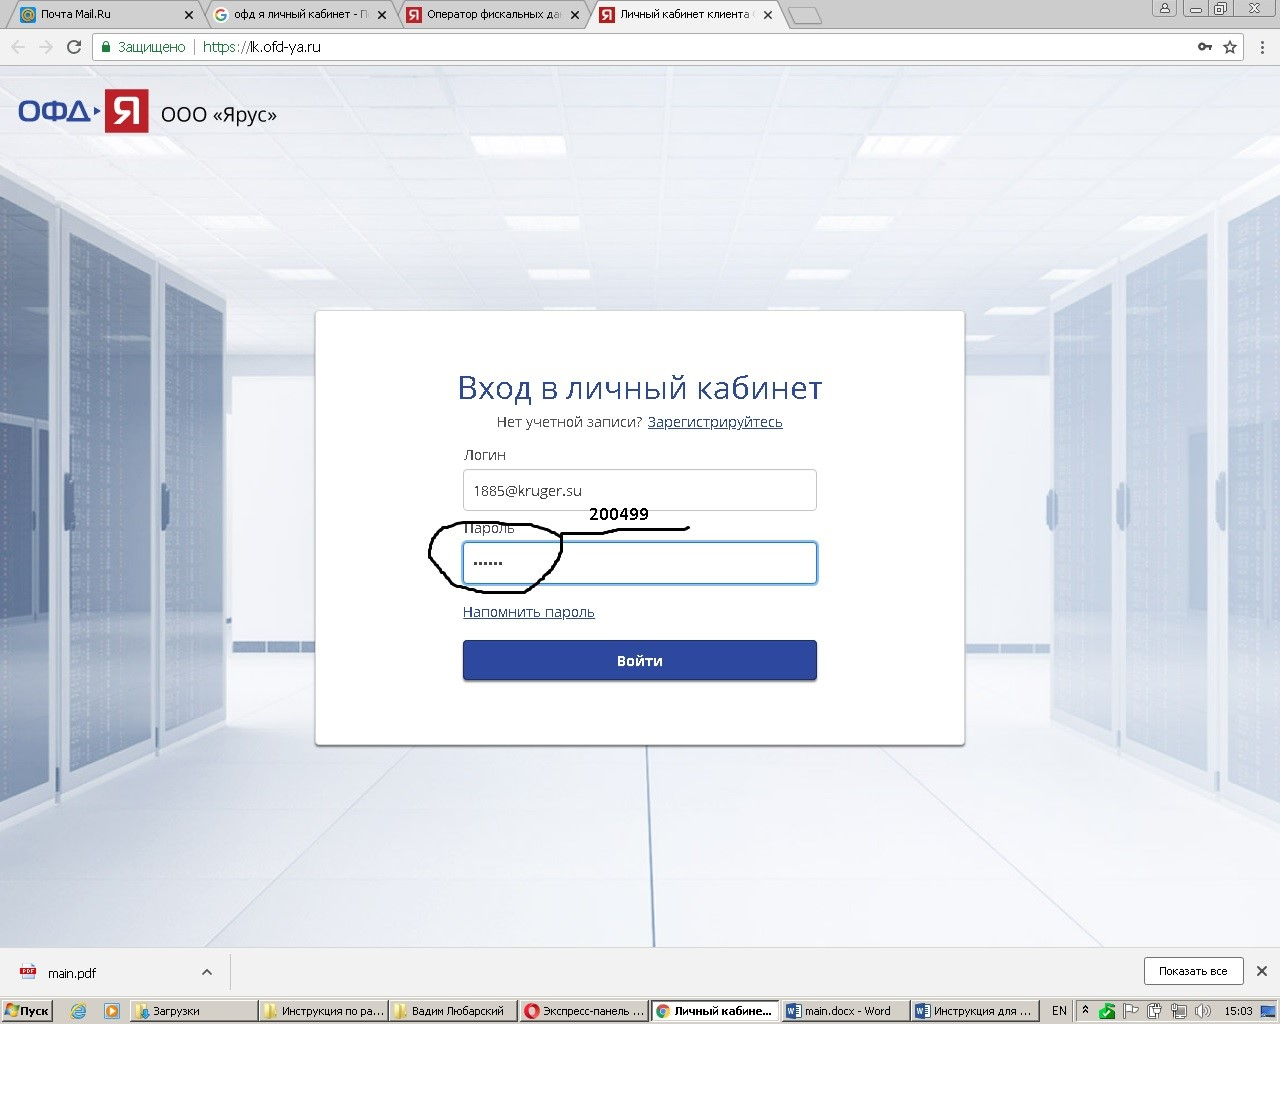
\includegraphics[width=1.0\textwidth]{15.jpg}
		\caption{<<Логин, пароль>>.}
		\label{ris:15.jpg}
	\end{figure}
	
	
	
	\item В открывшемся окне (Рис.~\ref{ris:16.jpg}) для ускорения поиска нужного чека можно установить отбор по дате, по конкретной торговой точке и по конкретной кассе. Искать нужный чек можно по сумме или по номеру чека. Номер чека это колонка «Порядковый номер ФД». Номер чека в этой колонке совпадает с номером чека в программе «1С».
	
	\begin{figure}[H]
		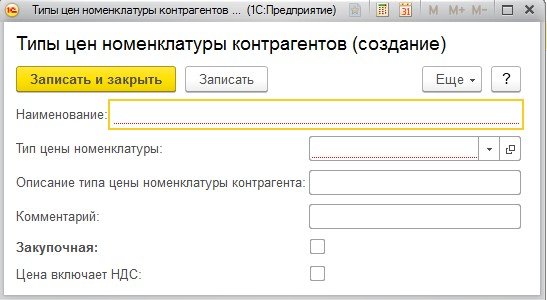
\includegraphics[width=1.0\textwidth]{16.jpg}
		\caption{<<Сайт ОФД>>.}
		\label{ris:16.jpg}
	\end{figure}

	\item Для того, что бы узнать содержимое чека, необходимо дважды кликнуть по строке с нужным чеком. Откроется его содержимое. (Рис.~\ref{ris:17.jpg})
	

	\begin{figure}[H]
		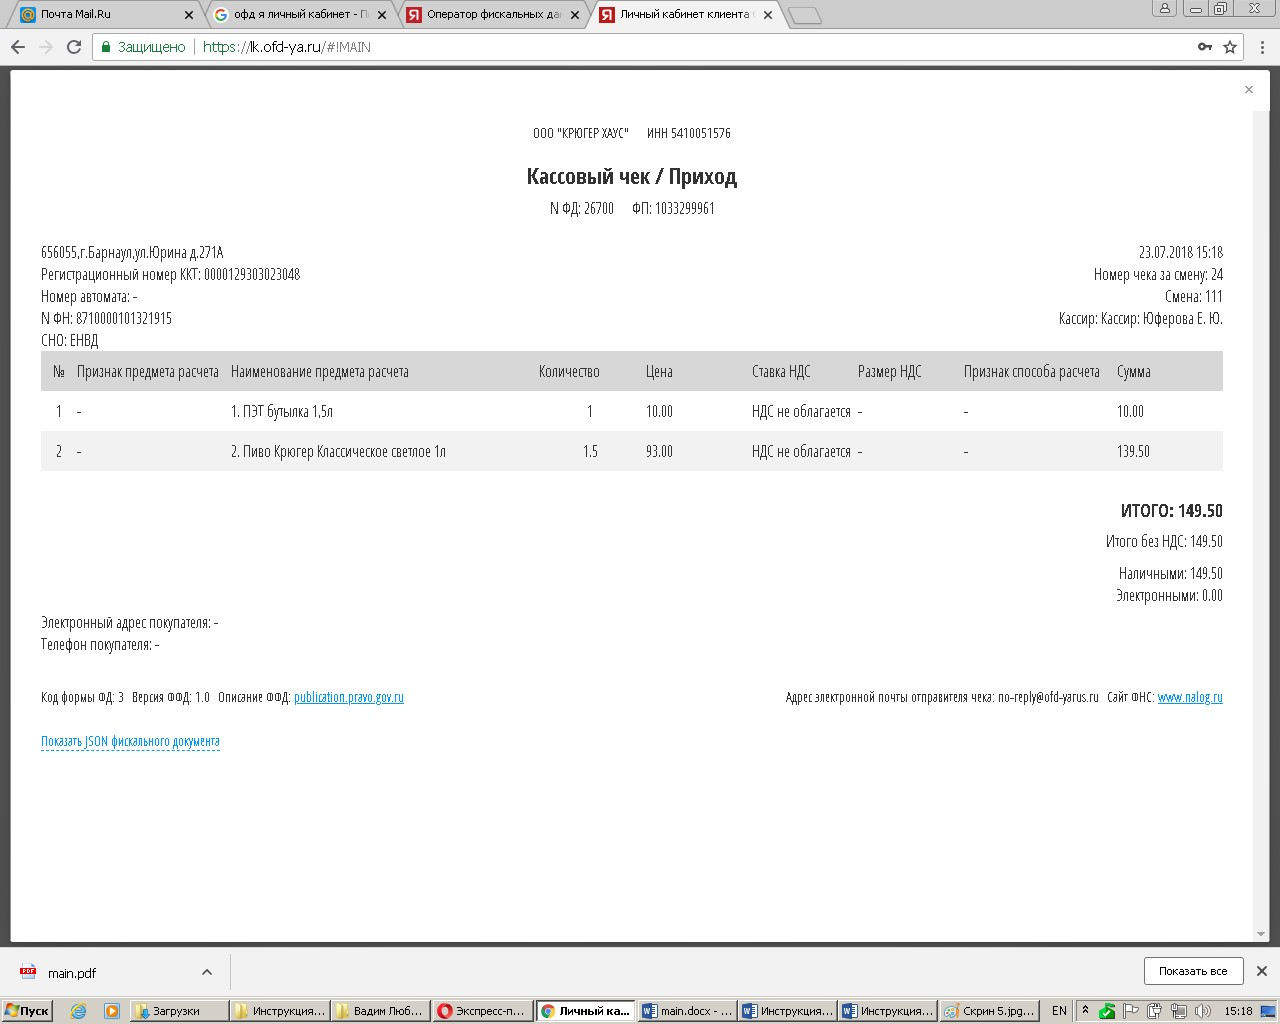
\includegraphics[width=1.0\textwidth]{17.jpg}
		\caption{<<Чек>>.}
		\label{ris:17.jpg}
	\end{figure}
	
	
	
\end{itemize}
